\documentclass{article}
\usepackage[margin=1in]{geometry}
\usepackage{minted}
\usepackage{xcolor}
\definecolor{LightGray}{gray}{0.90}
\usepackage[explicit]{titlesec}
\usepackage{amsmath}
\usepackage{nameref}
\usepackage[colorlinks=true]{hyperref}
\usepackage{textcomp} %For adding < >
\usepackage{graphicx}
\usepackage{listings}

\titleformat{\section}{\normalfont\Large\bfseries}{}{0em}{#1} %add this after #1 to include section number\ \thesection}


\title{Python Portfolio}
\author{Herman D. Schaumburg}

\date{\today} 

%This didn't work:
%\newenvironment{pythoncode}
%{ \begin{minted}[frame=lines,framesep=2mm,baselinestretch=1.2,bgcolor=LightGray,fontsize=\footnotesize,linenos]{python} }
%{ \end{minted} }

\newminted[pythoncode]{python}{frame=lines,framesep=2mm,baselinestretch=1.2,bgcolor=LightGray,fontsize=\footnotesize,linenos}

\newcommand{\mintedpython}[1]{\inputminted[frame=lines,framesep=2mm,baselinestretch=1.2,bgcolor=LightGray,fontsize=\footnotesize,linenos]{python}{#1}}



\begin{document}
\setlength{\parindent}{0pt}


\maketitle

\begin{abstract}
Here are some examples of my Python codes.  Included are  \nameref{sec:scikit} \nameref{sec:pand}, \nameref{sec:py_chal}, and \nameref{sec:matplotlib}.  I also include some problem statements and descriptions of how the codes and solutions work.  I may add more to this and post them \href{https://drive.google.com/drive/folders/1TfQg_Ua7G6nESDf_iinJsPVJzF_vYCEA?usp=sharing}{here}.  The python scripts with data files are also located within this directory.  All files may be downloaded in the Python{\_}Portfolio.zip file.
\end{abstract}

\section{Scikit-learn example: credit card fraud}
\label{sec:scikit}

\subsection{Origin and data set}
For this example, I followed the tutorial found at the URL below and added some code to measure the accuracy of predictions made by three estimators (Naive Bayes, LinearSVC, and K-Neighbors Classifier).  

\href{https://www.dataquest.io/blog/sci-kit-learn-tutorial/}{https://www.dataquest.io/blog/sci-kit-learn-tutorial/}

\bigskip
Based on the machine{\_}learning{\_}map found at the URL below, I should have tried SVC or Ensemble Classifiers instead of Naive Bayes.

\href{https://scikit-learn.org/stable/tutorial/machine_learning_map/}{https://scikit-learn.org/stable/tutorial/machine{\_}learning{\_}map/}

\bigskip
I choose to use a credit card fraud data set from kaggle instead of the one in the tutorial.  The columns of the transaction data set are Time (time elapsed from first transaction to current one), V1, V2, \dots, V28, Amount, and Class.  The class indicates if the transaction was a fraud Class=1 or not Class=0.  The V's are a result of applying Principal Component Analysis (PCA).   

\href{https://www.kaggle.com/mlg-ulb/creditcardfraud}{https://www.kaggle.com/mlg-ulb/creditcardfraud}

\bigskip
The script below employs \texttt{train{\_}test{\_}split} to split the data into training and testing components.  I used 70\% of the data for training and 30\% for testing.  I first used all the data in its raw form for the task and then compared this to a few other strategies.  Since the data set has 492 frauds out of 284,807 transactions, .  The script I wrote follows:

\subsection{code}
\mintedpython{Scikit-learn_credit_card_fraud/ml_credit_card_fraud.py}

\subsection{Results}
LinearSVC gave convergence warnings with max{\_}iter=1000 and max{\_}iter=1500.  I settled on setting this option \texttt{dual=False} in LinearSVC, which I need to understand further.

\bigskip
The script above uses the columns Time, V1, V2, \dots, V28, Amount for the training data.  Running the script gave this result:
\begin{lstlisting}
*** Naive-Bayes Estimater Results ***
Length of target data  85443
Number of predictions made:  85443
Number of frauds committed:  141
Number of frauds caught:  91
Number of false positives:  585
Number of false negatives:  50
Naive-Bayes accuracy :  0.9925681448451014
*** LinearSVC Results ***
Length of target data  85443
Number of predictions made:  85443
Number of frauds committed:  141
Number of frauds caught:  86
Number of false positives:  12
Number of false negatives:  55
LinearSVC accuracy :  0.9992158515033414
*** K-Neighbors Classifier Results ***
Length of target data  85443
Number of predictions made:  85443
Number of frauds committed:  141
Number of frauds caught:  22
Number of false positives:  1
Number of false negatives:  119
K-Neighbors Classifier accuracy :  0.9985955549313578
\end{lstlisting}
Removing the Time column made sense to me since there is no way to tell if the transactions were from the same account.  The only change in the script was changing line 17 to \texttt{col{\_}labels=col{\_}labels[1:len(col{\_}labels)-1]}. Of the three ways I considered the Time column, this way worked produced the best results.  Dropping Time from the dataset gave these results:
\begin{lstlisting}
*** Naive-Bayes Estimater Results ***
Length of target data  85443
Number of predictions made:  85443
Number of frauds committed:  141
Number of frauds caught:  120
Number of false positives:  1900
Number of false negatives:  21
Naive-Bayes accuracy :  0.9775171751928186
*** LinearSVC Results ***
Length of target data  85443
Number of predictions made:  85443
Number of frauds committed:  141
Number of frauds caught:  82
Number of false positives:  10
Number of false negatives:  59
LinearSVC accuracy :  0.9991924440855307
*** K-Neighbors Classifier Results ***
Length of target data  85443
Number of predictions made:  85443
Number of frauds committed:  141
Number of frauds caught:  94
Number of false positives:  6
Number of false negatives:  47
K-Neighbors Classifier accuracy :  0.9993797034280163
\end{lstlisting}

The Naive-Bayes caught more frauds, but had a much larger number of false positives than before. LinearSVC caught fewer frauds and K-Neighbors Classifier caught many more frauds and had only 6 false positives.  

\bigskip
In this test, I replaced the Time column with the increment of time between the current transaction and the previous one.  There was a substantial increase in runtime with slightly different results.  The Naive-Bayes had a higher number of false positives.
\begin{lstlisting}
*** Naive-Bayes Estimater Results ***
Length of target data  85443
Number of predictions made:  85443
Number of frauds committed:  141
Number of frauds caught:  120
Number of false positives:  2001
Number of false negatives:  21
Naive-Bayes accuracy :  0.976335100593378
*** LinearSVC Results ***
Length of target data  85443
Number of predictions made:  85443
Number of frauds committed:  141
Number of frauds caught:  82
Number of false positives:  10
Number of false negatives:  59
LinearSVC accuracy :  0.9991924440855307
*** K-Neighbors Classifier Results ***
Length of target data  85443
Number of predictions made:  85443
Number of frauds committed:  141
Number of frauds caught:  93
Number of false positives:  7
Number of false negatives:  48
K-Neighbors Classifier accuracy :  0.9993562960102056
\end{lstlisting}

\section{Pandas coding challenge}
\label{sec:pand}

{\bf Dataset} The dataset ny-demographics.csv contains information on the residential demographics of each
census tract in New York state. The dataset contains the following variables:

\bigskip
\hspace*{\fill}
\begin{tabular}{ll}
geoid11 & 11-digit geographic identifier for census tract\\
geoid11name & Name of census tract, county, and state\\
population & Number of residents in census tract\\
asian & Number of tract residents who are non-Hispanic Asians\\
black & Number of tract residents who are non-Hispanic blacks\\
hispanic & Number of tract residents who are Hispanic\\
white & Number of tract residents who are non-Hispanic whites\\
\end{tabular}
\hspace*{\fill}

\bigskip
A row in the dataset describes one census tract. For example, the row that begins

\bigskip
\hspace*{\fill}
\begin{tabular}{ll}
geoid11 & geoid11name\\
36001000100 & Census Tract 1, Albany County, New York
\end{tabular}
\hspace*{\fill}

\bigskip
indicates that there are 2139 residents in Census Tract 1 of Albany County, New York, of whom
55 are non-Hispanic Asians.
There are 4919 census tracts in New York state and there are no missing values in the dataset.
The “geoid11” variable has the property that the first 2 digits identify the state (36 = New York)
and the first 5 digits identify the county within the state (36001 = Albany, New York). Tracts
partition a county: if you add up all the residents in the 75 tracts in Albany County, this equals the
population of Albany County (304,204 residents). There are nine tracts in which the population
variable is the population count followed by “(rXXXXX)”, where XXXXX is a 5-digit revision
number, indicating that the Census Bureau revised the population count at some point after the
initial data release.

\bigskip
{\bf Task} Your assignment is to write a short script that generates a county-level dataset describing each
New York county's demographics. In particular, please produce a CSV file containing the following
variables:

\bigskip
\begin{tabular}{ll}
geoid5 & 5-digit geographic identifier for county\\
geoid5name & Name of county and state\\
population & Number of residents in county\\
asian share & Fraction of county residents who are non-Hispanic Asians\\
black share & Fraction of county residents who are non-Hispanic blacks\\
hispanic share & Fraction of county residents who are Hispanic\\
white share & Fraction of county residents who are non-Hispanic whites\\
tracts & Number of census tracts in county\\
asian majority tracts & Number of tracts in county where $>$ 50\% of residents are non-Hispanic Asians\\
black majority tracts & Number of tracts in county where $>$ 50\% of residents are non-Hispanic blacks\\
hispanic majority tracts & Number of tracts in county where $>$ 50\% of residents are Hispanic\\
white majority tracts & Number of tracts in county where $>$ 50\% of residents are non-Hispanic whites\\
nomajority tracts & Number of tracts in county where no demographic category has $>$ 50\% share
\end{tabular}

\bigskip
The dataset should include one observation for each of New York's 62 counties and should be
sorted by the 5-digit code that identifies the county. If you need to make judgment calls about how
to process the data, please write us a short note describing the decisions you made.

\bigskip

{\it Solution: }Assumptions:
\begin{itemize}
\item The demographics are based on the unrevised populations.  (I based this on line 375 where the revised population is more than 10X the sum of the ethnic populations)
\item I assumed that I should count any tract(s) with no one living in them.
\end{itemize}

\bigskip
The python script outputs two csv files with revised and unrevised numbers in the populations collumn.  

\mintedpython{Pandas_coding_challenge/task1.py}

%\section{Householder Transformation}

%\section{Classical numerators}





\section{Python coding challenge}
\label{sec:py_chal}

The following are my solutions to problems posed in a coding challenge.

{\bf Problem 1} On Pandora, the currency is called Unob, U. There are six coins in circulation:
\[\text{U1, U5, U10, U20, U50, U100}\]

It is possible to make U500 in the following way:

\[3\times\text{U}100 + 2\times\text{U}50 + 4\times\text{U}20 + 1\times\text{U}10 + 1\times\text{U}5 + 5\times\text{U}1\]

How many different ways can U500 be made using any number of coins?

\bigskip
{\it Solution:} I used a generating function to solve this problem.  A generating function is a power series
\[g(x)=\sum_{j=0}^\infty A_n x^n,\]
where $A_n$ counts some set.  An example relevant to the solution is the number of ways to write an integer $n$ as a sum of integers $1$ or $5$ where order is irrelevant.  The generating function is
\begin{align}
h(x)=(1+x+x^{1+1}+x^{1+1+1}+\cdots)(1+x^5+x^{5+5}+x^{5+5+5}+\cdots) \label{eqn:gf1}\\
=\frac{1}{1-x}\frac{1}{1-x^5}. \label{eqn:gf2}
\end{align}
The fact that the two factors on the right hand side of \eqref{eqn:gf1} are geometric series gives \eqref{eqn:gf2}.  To understand this generating function consider the case where $n=15$ the following make contributions to the coefficient of $x^11$:
\[x^{1+1+1+1+1+1+1+1+1+1+1} \quad   x^{1+1+1+1+1+1+5}\quad   x^{1+5+5}. \]
The exponents correspond to the three ways to make U15 from U1 and U5 coins.  The following Python script gives the 500th coefficient of the generating function of 
\[f(x)=\frac{1}{(1-x)(1-x^5)(1-x^{10})(1-x^{20})(1-x^{50})(1-x^{100})},\]
which is the answer for this problem.


\mintedpython{Python_coding_challenge/problem1.py}

{\bf Problem 2} 
\begin{itemize}
\item Gregor has eight five-sided dice, each with faces numbered 1, 2, 3, 4, 5.
\item Oberyn has four ten-sided dice, each with faces numbered 1, 2, 3, 4, 5, 6, 7, 8, 9, 10.
\end{itemize}
Gregor and Oberyn roll their dice and compare totals: the highest total wins. The result is a draw if the
totals are equal.
What is the probability that Gregor beats Oberyn (i.e. Gregor wins / N games)?

\bigskip
{\it Solution:} The idea for my solution is to find the sum
\[ \sum_{i=9}^{40} (\text{Number of ways Oberyn rolls sum to}<i) \times (\text{Number of ways Gregor rolls sum to }i)\]
and divide by the number of games, which is 
\[5^8 \times 10^4.\]

The part of the solution involving Oberyn is computed according using
\[\text{Number of ways Oberyn rolls sum to }<i=\sum_{j=4}^i (\text{Number of ways Oberyn rolls sum to }j).\]

The solution be completed by finding the number of ways an $M$ sided dice sums to $n$.  That is the problem we need to solve is

\hspace*{\fill} {\bf (I)} \hspace*{0.5in} \begin{minipage}{0.5\textwidth}
 Find the number of solutions to
\[x_1+x_2+\dots+x_k=n\]
where $1 \leq x_j\leq M$.
\end{minipage}
\hspace*{\fill}

This is related to problem 

\hspace*{\fill} {\bf (II)} \hspace*{0.5in} \begin{minipage}{0.5\textwidth}
 Find the number of solutions to
\[y_1+y_2+\dots+y_k=n\]
where $1 \leq x_j $.
\end{minipage}
\hspace*{\fill}

whose solution is the binomial coefficient $_{n-1}C_{k-1}$, $n-1$ choose $k-1$.  This fact may be understood by considering $M$ ones with wedges $\wedge$ between them
\[1 {_\wedge} 1 {_\wedge} 1 {_\wedge} 1 {_\wedge} \cdots {_\wedge} 1.\]
Each wedge may is a place where one of $k-1$ plus signs may be placed.  The number of ones between plus signs correspond to the numbers $y_j$.  The number of ways to choose which of the $n-1$ wedges get one of the $k$ plus signs is $_{n-1}C_{k-1}$.  

\bigskip
Let $A_p$ be the number of solutions to {\bf (II)} where at least $p$ of the $y_j$ are greater than $M$.  From the principle of inclusion and exclusion the solution to problem {\bf (I)} is
\[_{n-1}C_k +\sum_{p>1} (-1)^p A_p \]
If we subtract $M$ from each of the $p$ integers that are greater than $M$, we see that $A_p$ is the solutions to problem {\bf (II)} with $n-pM$ substituted for $n$ times the number of ways to pick the $p$ integers that are greater from the $k$ integers.  Thus,
\[A_p=_k C _p \times _{n-pM-1} C _{k},\]
and
\[
\text{number of ways an }M\text{ sided dice sums to }n=_{n-1}C_k +\sum_{p>1} (-1)^p _k C _p \times _{n-pM-1} C _{k-1}.
\]
This is computed by the function \texttt{sum{\_}soln{\_}ct} in the python script below.  The script returns the answer
\[\frac{2278263384}{3906250000}=0.583235426304.\]

\bigskip
A potential area for improvement is to lower the number of flops to compute the the binomial coefficients by storing them in a table and using a recurrence formula to compute further rows. 

\mintedpython{Python_coding_challenge/problem2.py}

{\bf Problem 3} 
Problem 3.
Find the maximum value from the matrix where each number is the only one in its row and column. For
example, for the matrix below the maximum value equals 3315 ( = 863 + 383 + 343 + 959 + 767):

\hspace*{\fill}
\begin{tabular}{*{5}{c}}
7 & 53 & 183 & 439 & {\color{green} 863}\\
497 & {\color{green} 383} & 563 & 79 & 973\\
287 & 63 & {\color{green} 343} & 169 & 583\\
627 & 343 & 773 & {\color{green} 959} & 943\\
{\color{green} 767} & 473 & 103 & 699 & 303
\end{tabular}
\hspace*{\fill}

Find the maximum value of:

\begin{tabular}{*{15}{c}}
7 & 53 & 183 & 439 & 863 & 497 & 383 & 563 & 79 & 973 & 287 & 63 & 343 & 169 & 583\\
627 & 343 & 773 & 959 & 943 & 767 & 473 & 103 & 699 & 303 & 957 & 703 & 583 & 639 & 913\\
447 & 283 & 463 & 29 & 23 & 487 & 463 & 993 & 119 & 883 & 327 & 493 & 423 & 159 & 743\\
217 & 623 & 3 & 399 & 853 & 407 & 103 & 983 & 89 & 463 & 290 & 516 & 212 & 462 & 350\\
960 & 376 & 682 & 962 & 300 & 780 & 486 & 502 & 912 & 800 & 250 & 346 & 172 & 812 & 350\\
870 & 456 & 192 & 162 & 593 & 473 & 915 & 45 & 989 & 873 & 823 & 965 & 425 & 329 & 803\\
973 & 965 & 905 & 919 & 133 & 673 & 665 & 235 & 509 & 613 & 673 & 815 & 165 & 992 & 326\\
322 & 148 & 972 & 962 & 286 & 255 & 941 & 541 & 265 & 323 & 925 & 281 & 601 & 95 & 973\\
445 & 721 & 11 & 525 & 473 & 65 & 511 & 164 & 138 & 672 & 18 & 428 & 154 & 448 & 848\\
414 & 456 & 310 & 312 & 798 & 104 & 566 & 520 & 302 & 248 & 694 & 976 & 430 & 392 & 198\\
184 & 829 & 373 & 181 & 631 & 101 & 969 & 613 & 840 & 740 & 778 & 458 & 284 & 760 & 390\\
821 & 461 & 843 & 513 & 17 & 901 & 711 & 993 & 293 & 157 & 274 & 94 & 192 & 156 & 574\\
34 & 124 & 4 & 878 & 450 & 476 & 712 & 914 & 838 & 669 & 875 & 299 & 823 & 329 & 699\\
815 & 559 & 813 & 459 & 522 & 788 & 168 & 586 & 966 & 232 & 308 & 833 & 251 & 631 & 107\\
813 & 883 & 451 & 509 & 615 & 77 & 281 & 613 & 459 & 205 & 380 & 274 & 302 & 35 & 805
\end{tabular}

(Hint: the anser is $>13930$, you can implement the Hungarian Algorithm but it is not required)

\bigskip

{\it Solution:} The hint lead me to the name of a closely related problem, namely the assignment problem.  In the assignment problem, the minimum sum where where each summand is the only one in its row and column is returned.  Thus the solution to the problem at hand is given by
\[\text{solution for matrix } M=-\text{ solution of assignment problem for matrix }(-M)\] 
The script returns an answer of $13938$.  Uncommenting the line 18 gives the columns containing the summands which give this maximum sum, \texttt{[ 9 10  7  4  3  0 13  2 14 11  6  5 12  8  1]}.

\mintedpython{Python_coding_challenge/problem3.py}


\section{Matplotlib script}
\label{sec:matplotlib}

This plotting script takes files \texttt{x{\_}PHAD{\_}\textlangle{}index\textrangle{}.ssv} and \texttt{y{\_}PHAD{\_}\textlangle{}index\textrangle{}.ssv} then creates a series of density plots within a window specified by the ranges \texttt{xlims} and \texttt{ylims}. 

\bigskip
Below is a sample of a few plots created with this script.

\hspace*{\fill}
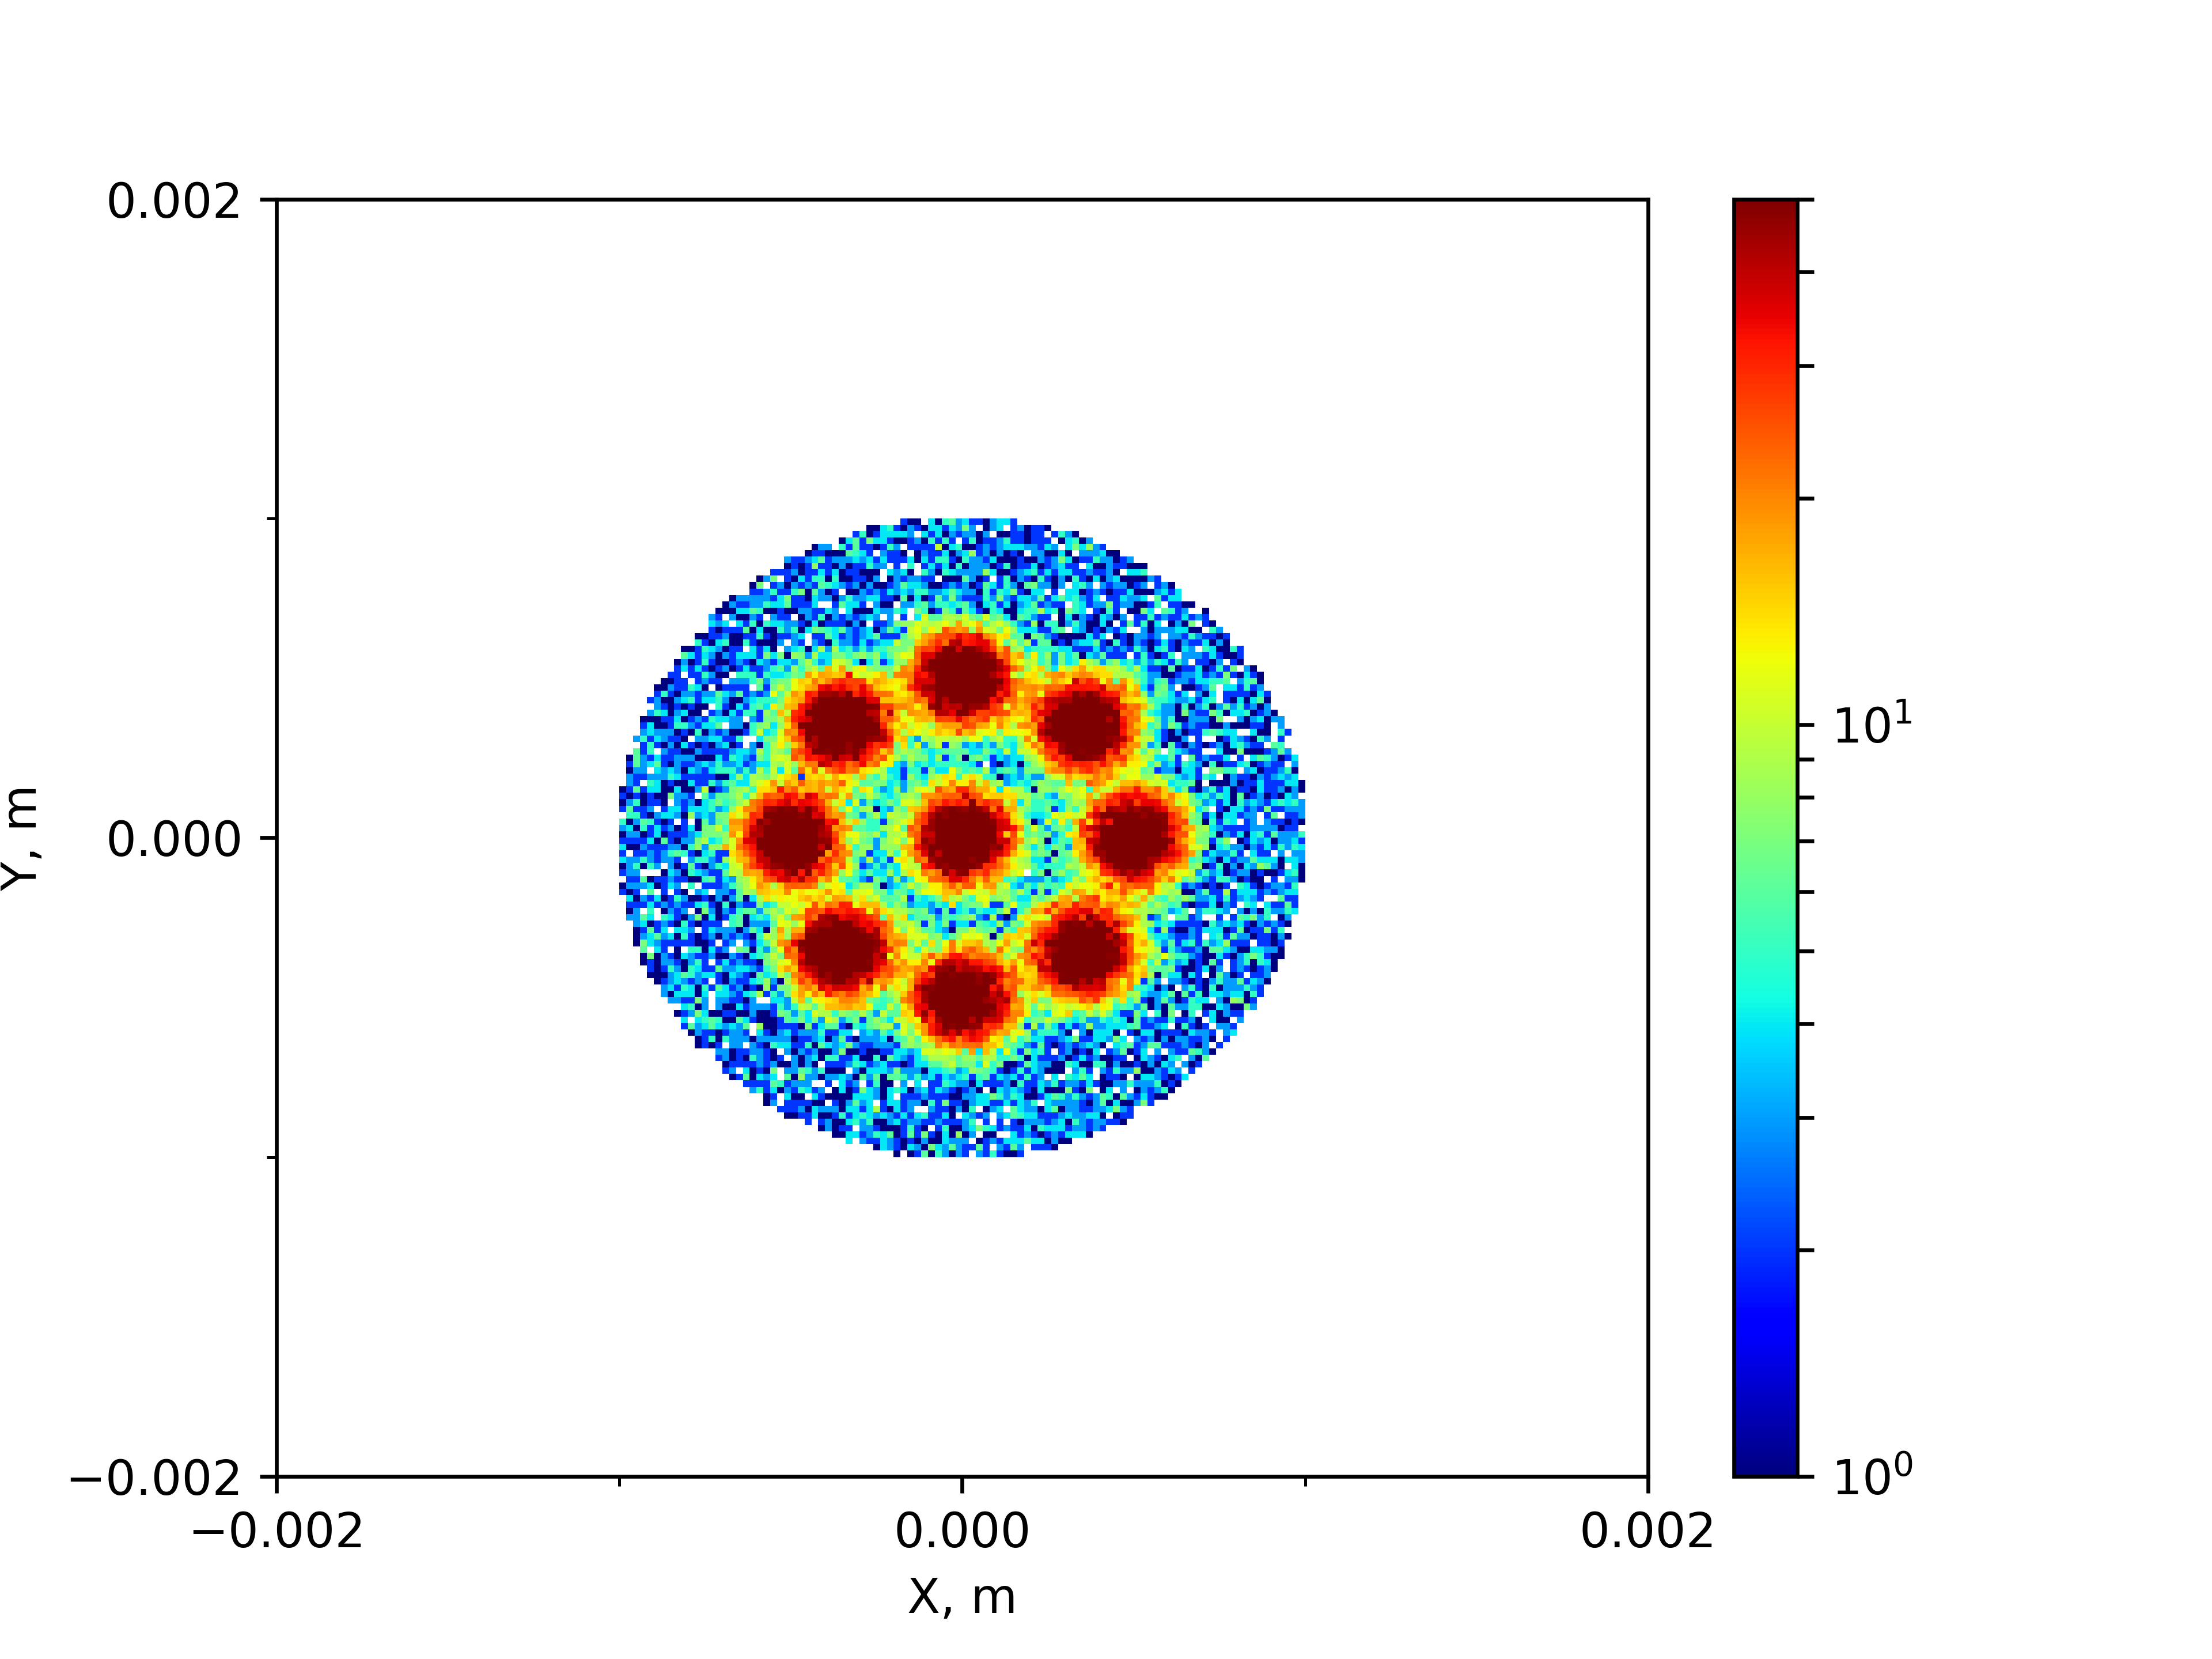
\includegraphics[scale=0.4]{Matplotlib_script/0000.png}
\hspace*{0.25in}
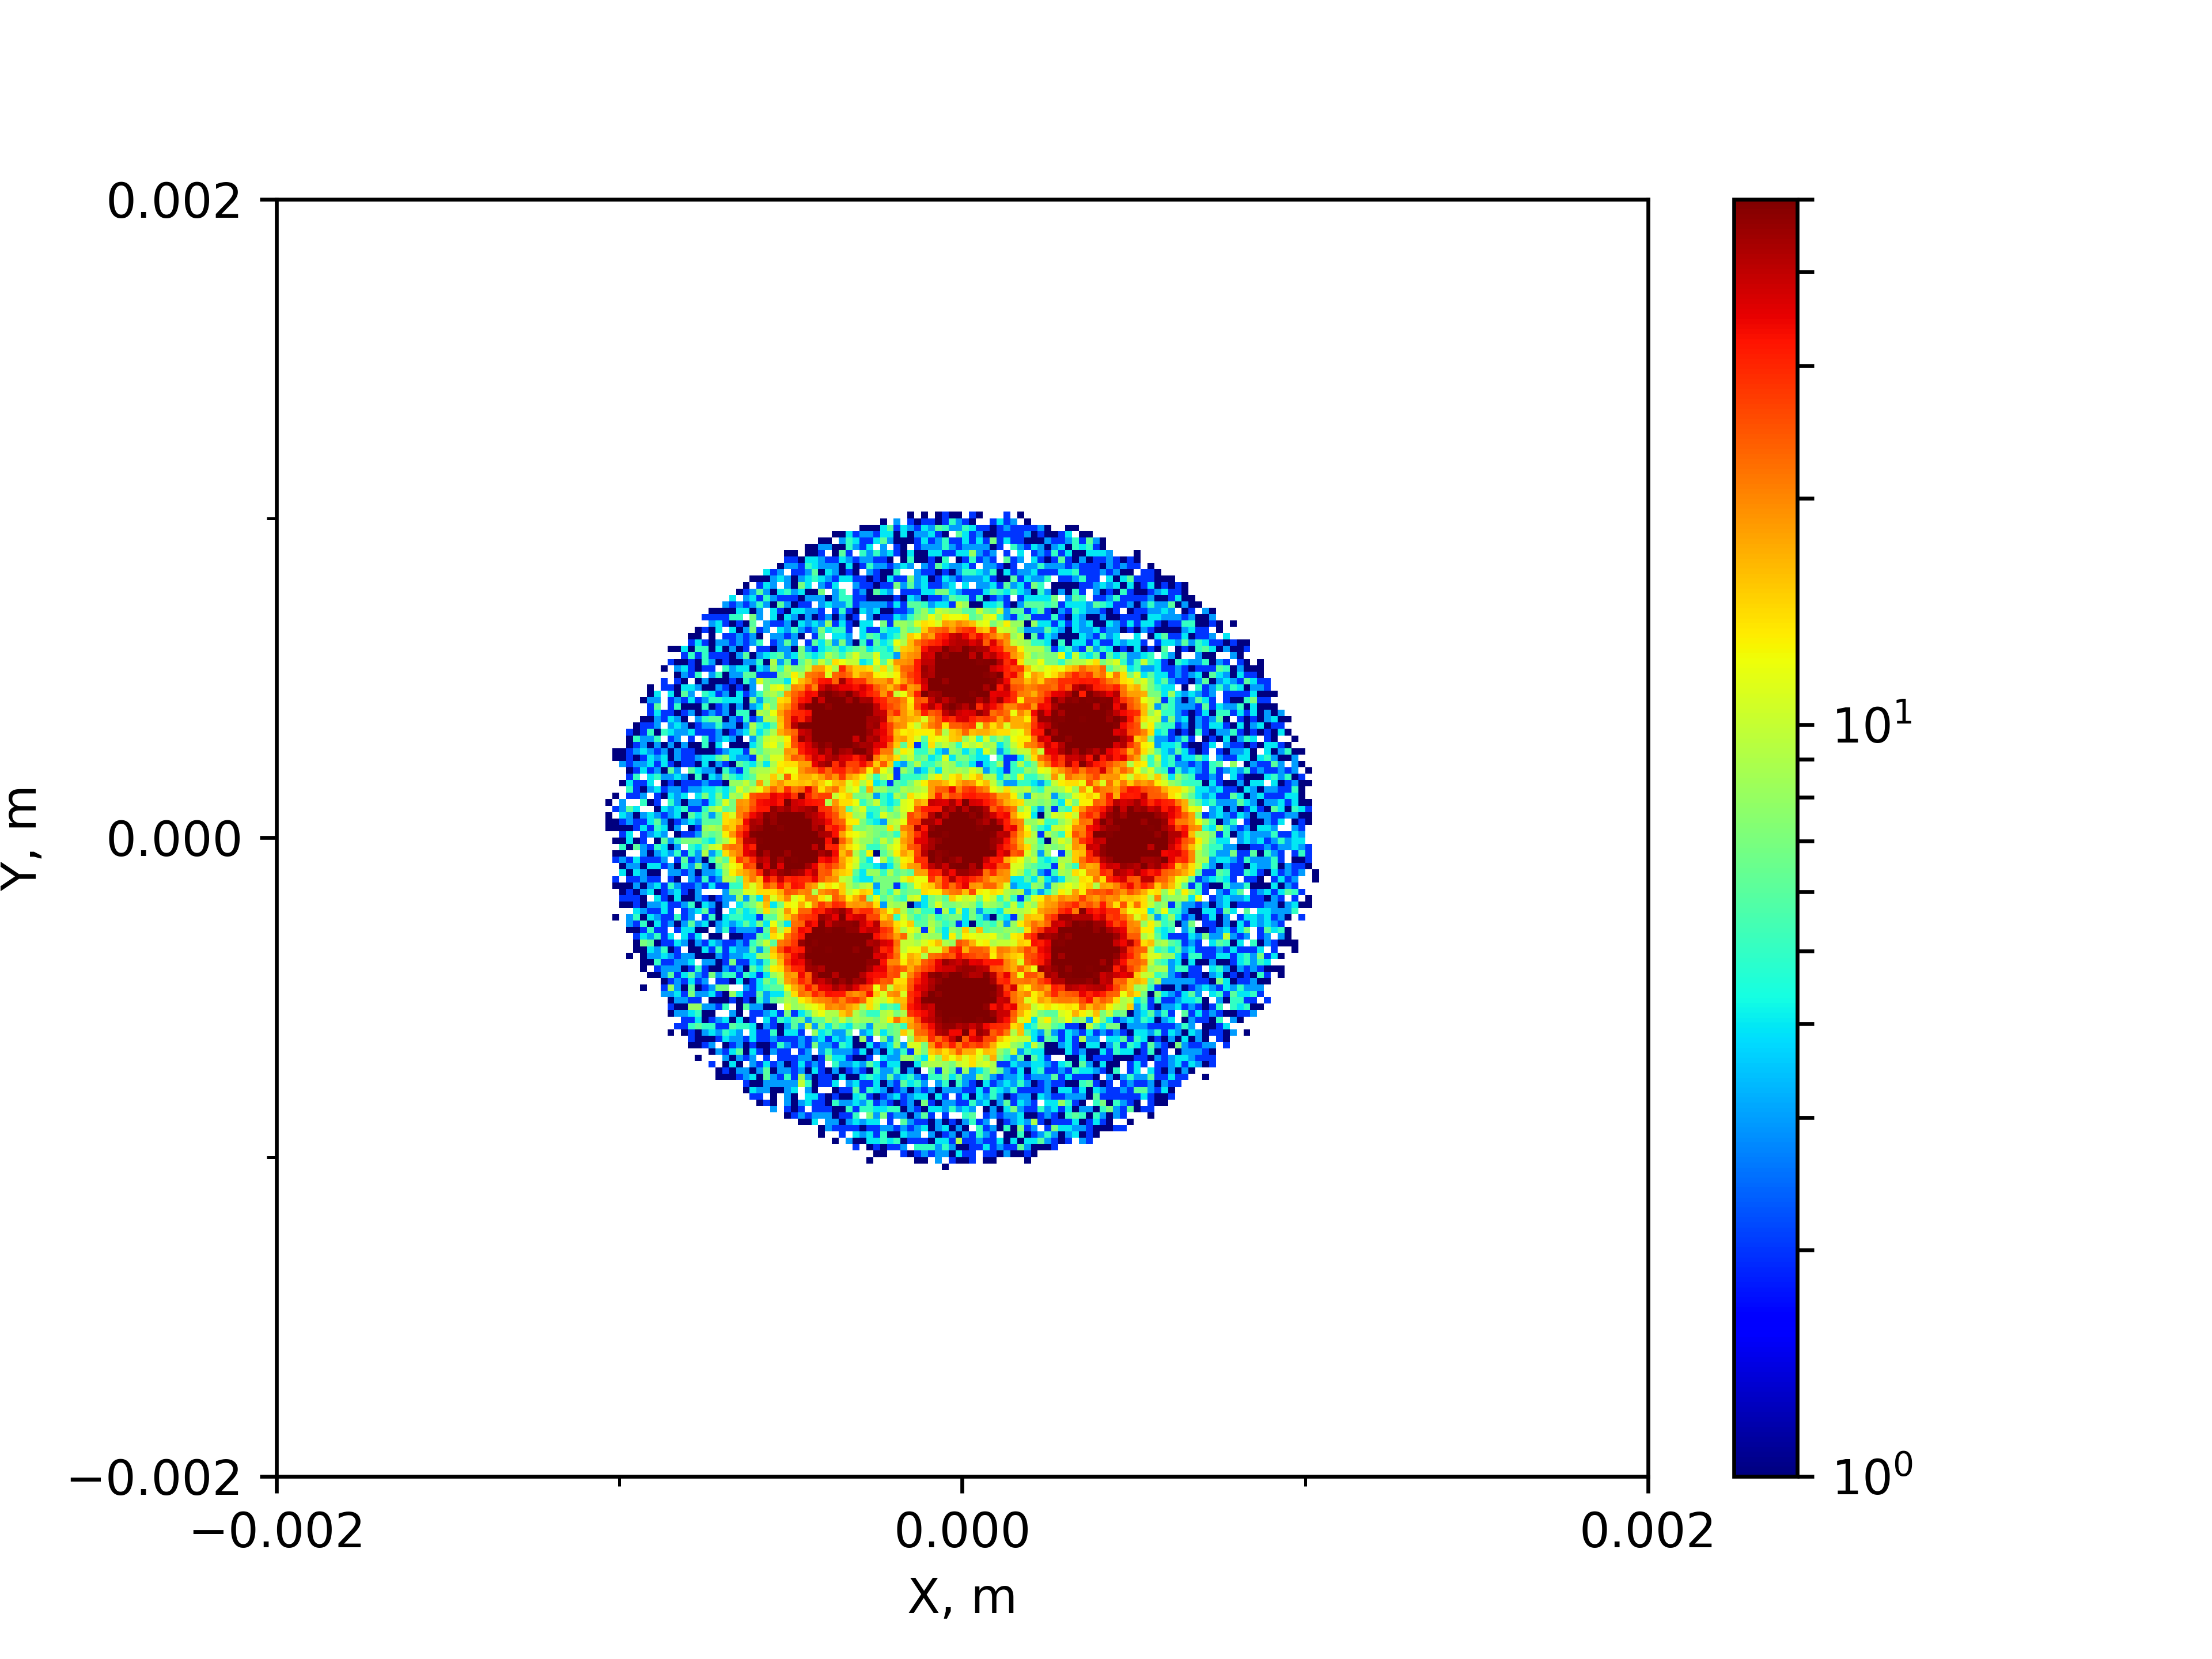
\includegraphics[scale=0.4]{Matplotlib_script/0001.png}
\hspace*{\fill}

\hspace*{\fill}
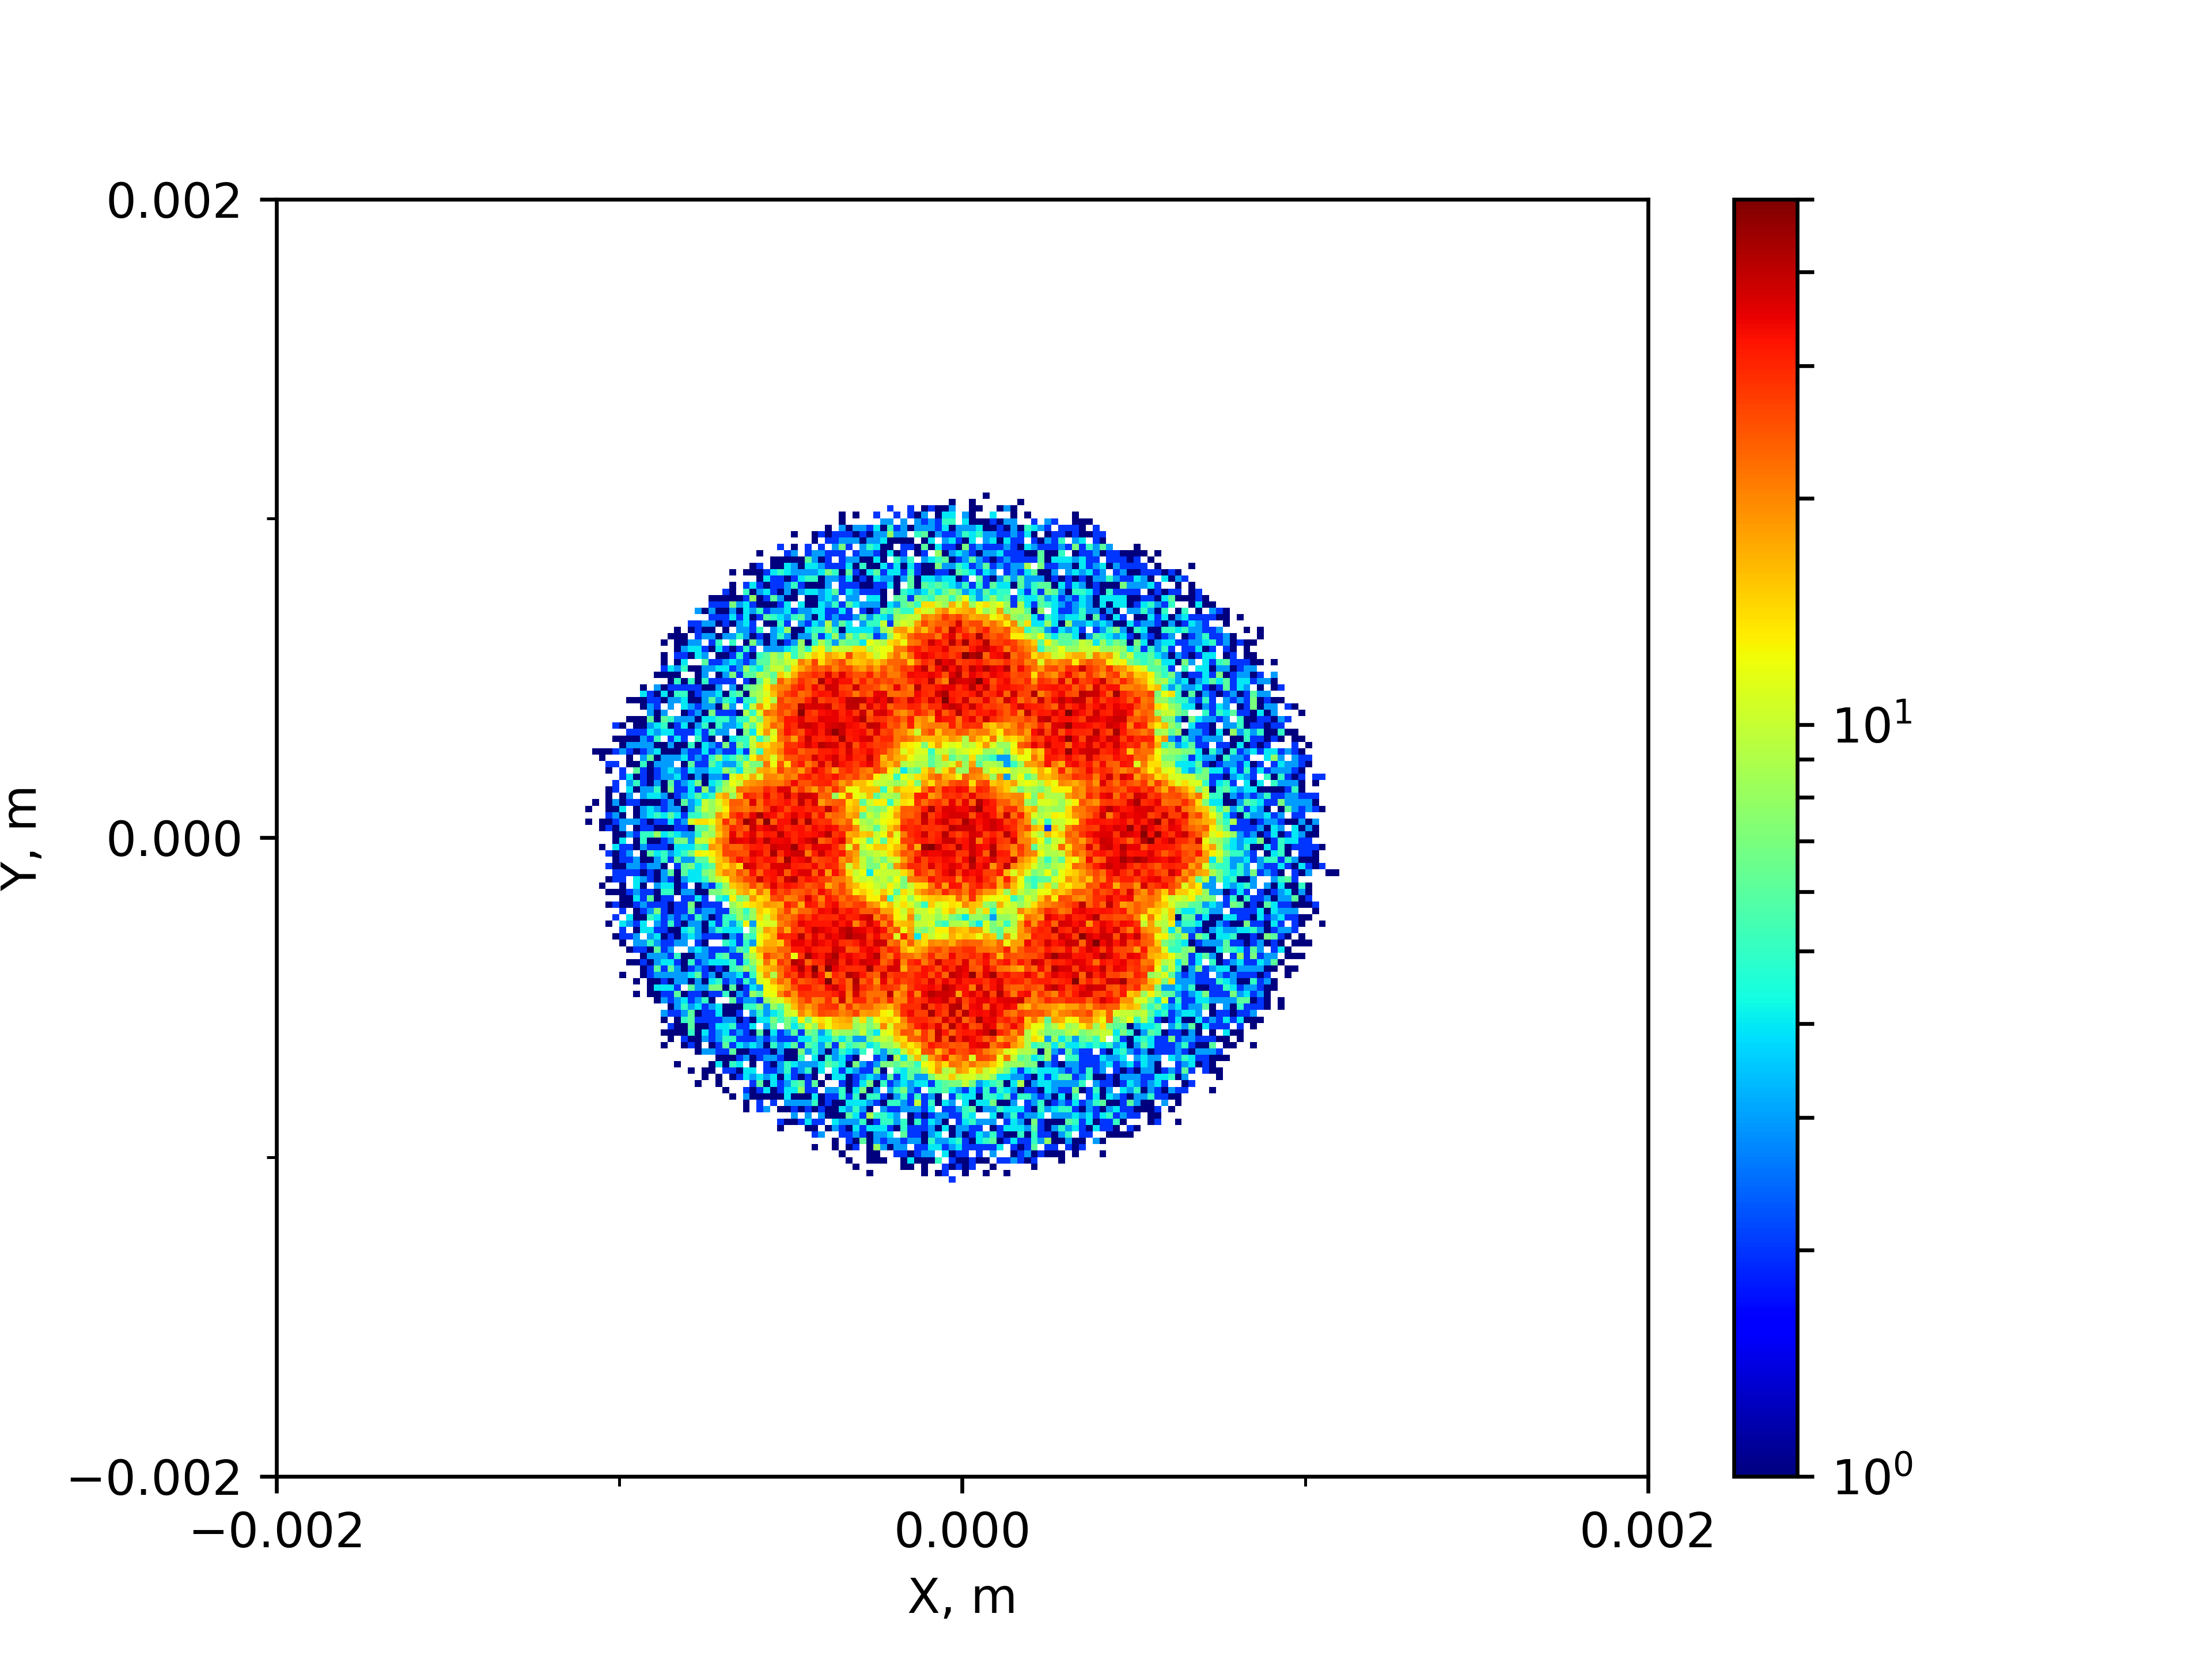
\includegraphics[scale=0.4]{Matplotlib_script/0002.png}
\hspace*{0.25in}
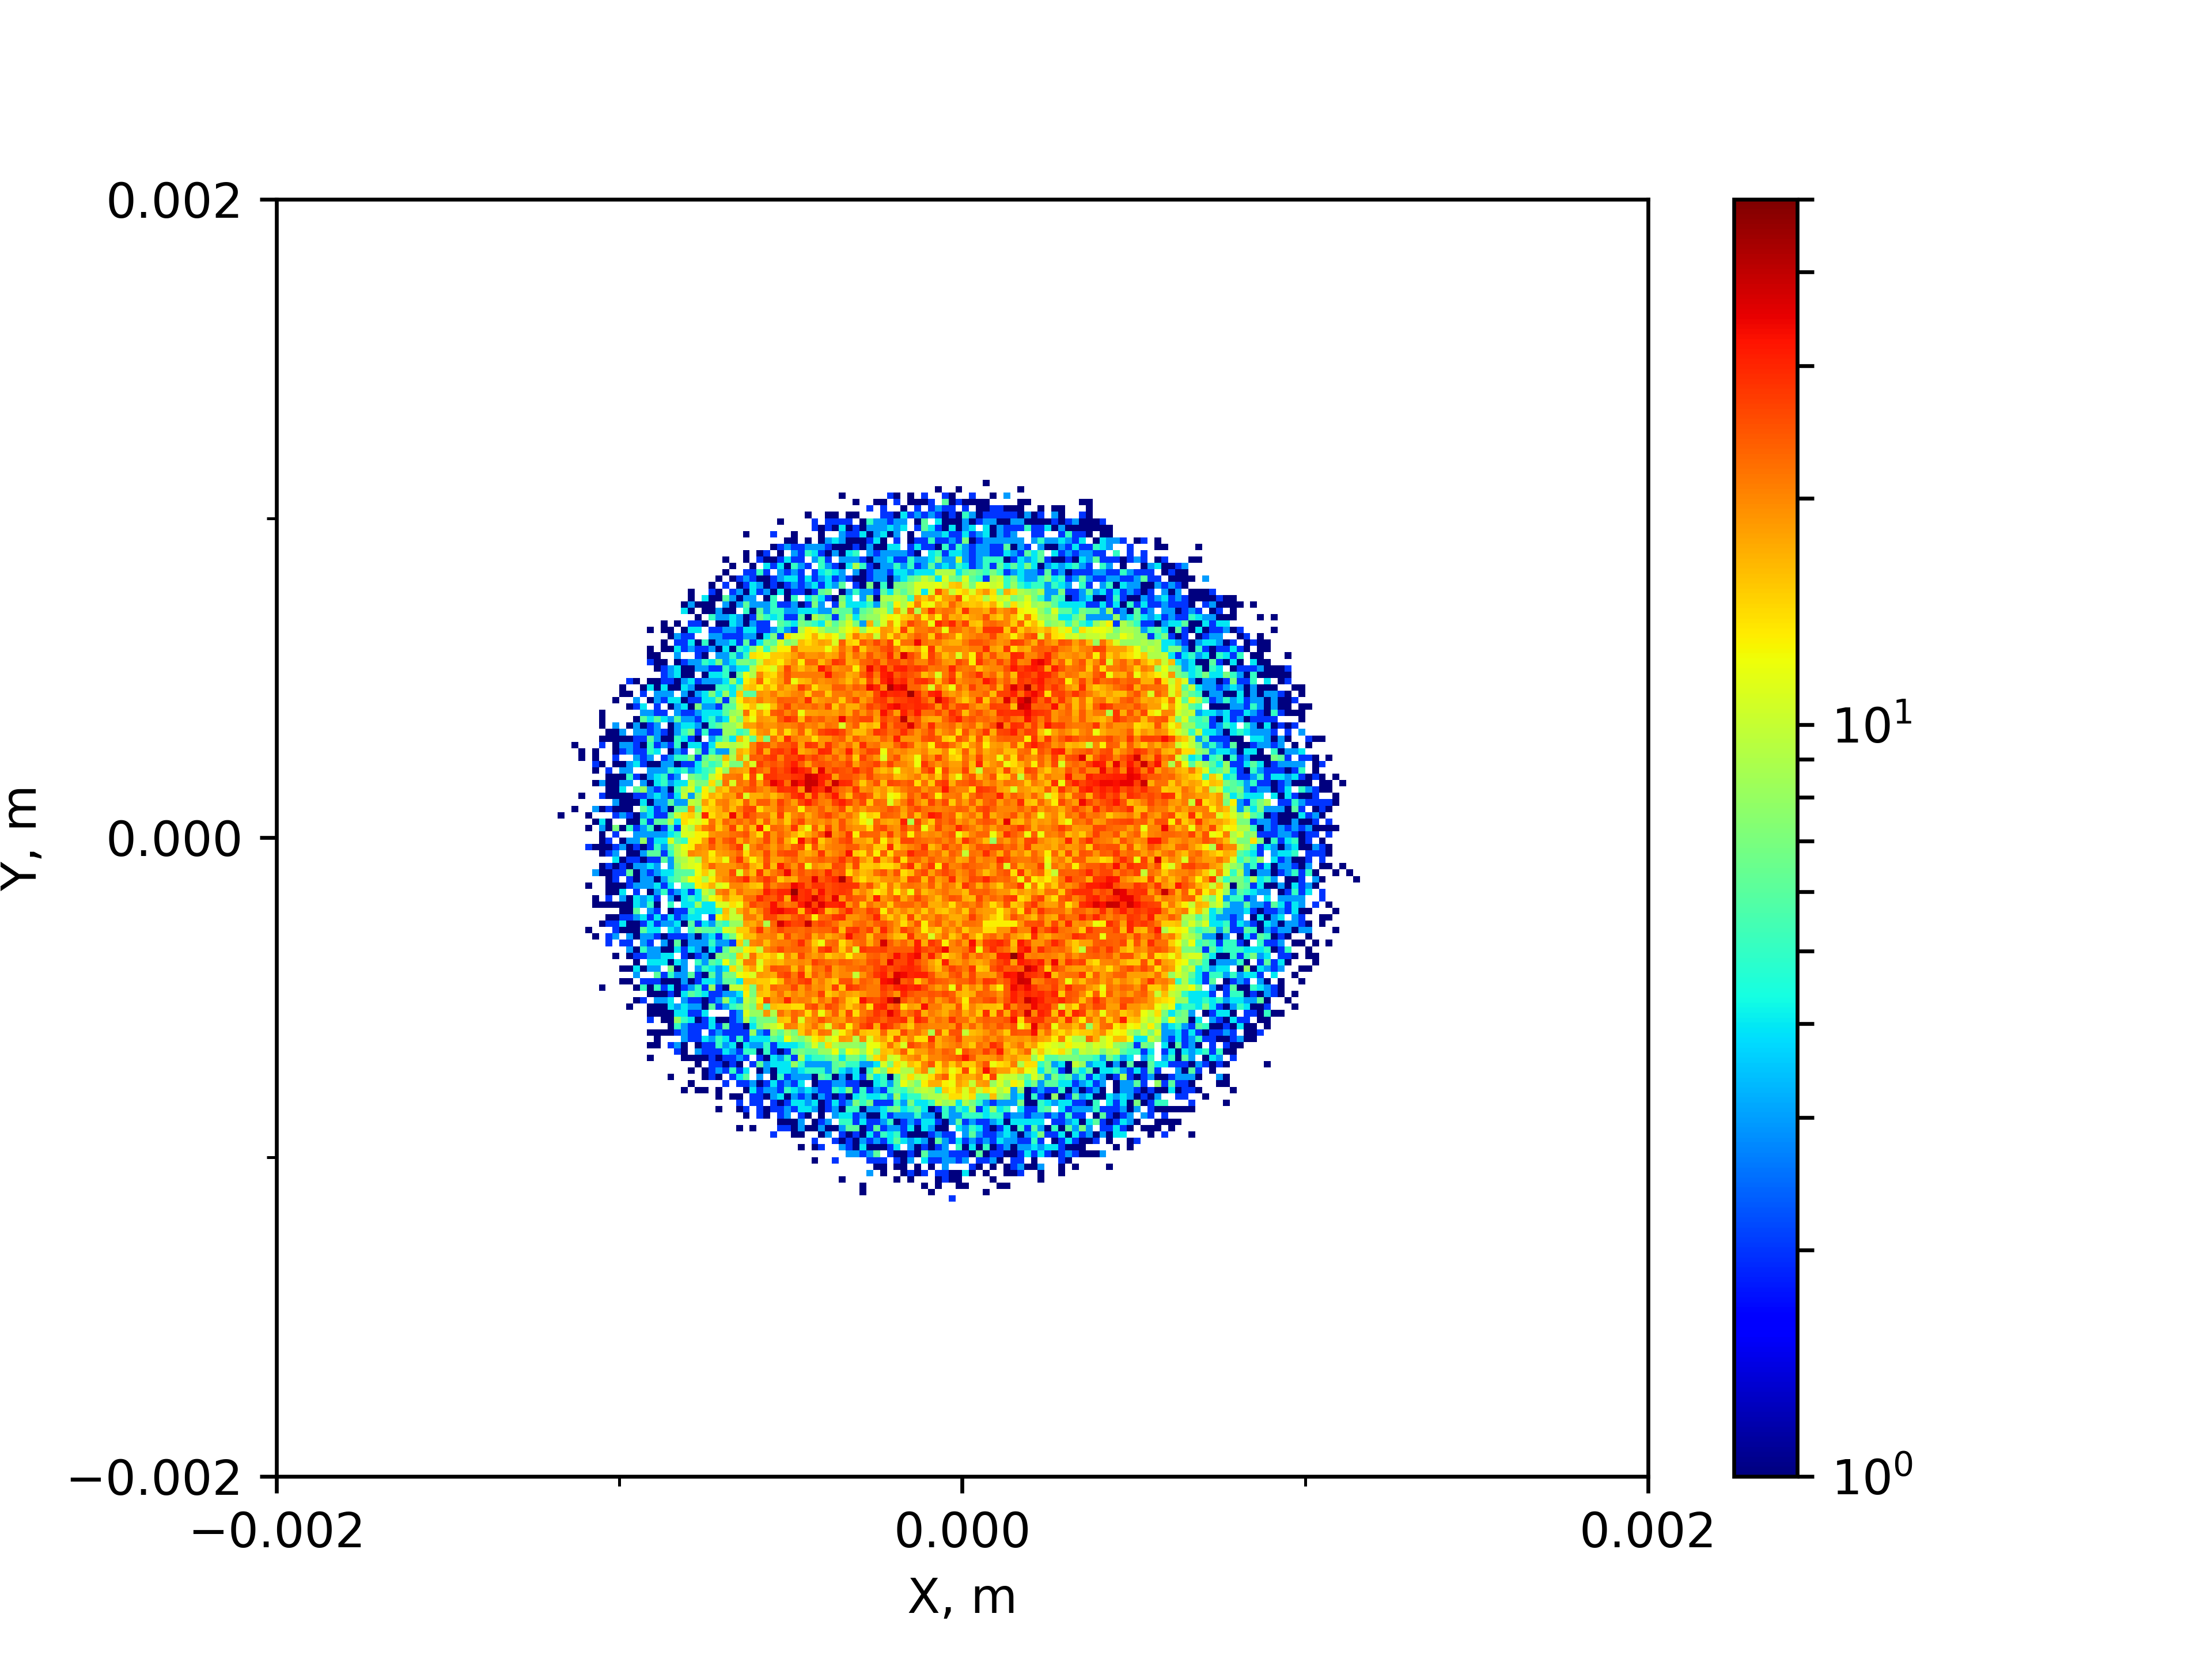
\includegraphics[scale=0.4]{Matplotlib_script/0003.png}
\hspace*{\fill}

An example animation created by different script that employed \LaTeX and imagemagik instead may be viewed \href{https://drive.google.com/file/d/1neBxOSLc-KTK15I5baHdyKoPCO4jqHwO/view}{here}.

\mintedpython{Matplotlib_script/density_plots_log.py}


\end{document}

\begin{pythoncode}

\end{pythoncode}